\begin{figure}
\center
\tiny

\pgfplotsset{width=\textwidth,height=6cm}
\pgfplotsset{every axis/.append style={
thick,
tick style={semithick}}}

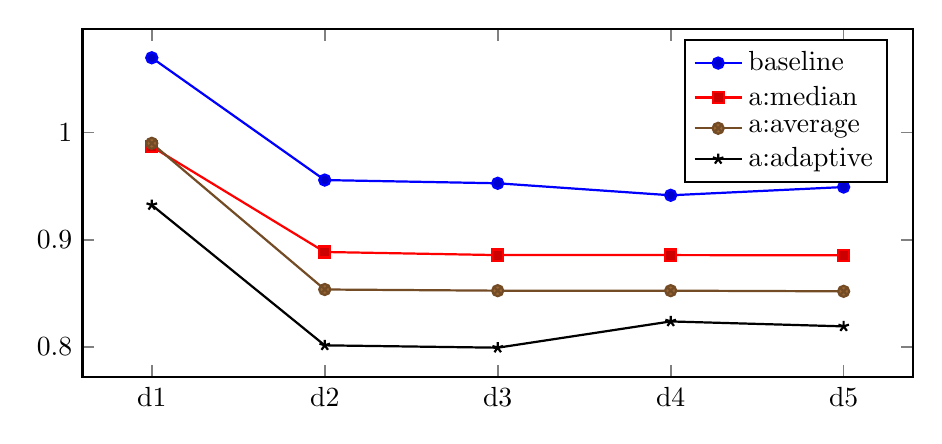
\begin{tikzpicture}

\begin{axis}[
  stack plots=false,
  enlarge x limits=true,
  symbolic x coords={d1,d2,d3,d4,d5},
  xtick=data,
  legend style={
    cells={anchor=west},
    legend pos=north east,
  }
]

\addplot coordinates {
(d1, 1.0698)
(d2, 0.9557)
(d3, 0.9527)
(d4, 0.9415)
(d5, 0.9492)
};
\addlegendentry{baseline}


\addplot coordinates {
(d1, 0.9869)
(d2, 0.8886)
(d3, 0.8857)
(d4, 0.8857)
(d5, 0.8855)
};
\addlegendentry{a:median}
 
\addplot coordinates {
(d1, 0.9900)
(d2, 0.8536)
(d3, 0.8525)
(d4, 0.8525)
(d5, 0.8519)
};
\addlegendentry{a:average}
 
\addplot coordinates {
(d1, 0.9324)
(d2, 0.8015)
(d3, 0.7993)
(d4, 0.8238)
(d5, 0.8192)
};
\addlegendentry{a:adaptive}

\end{axis}
\end{tikzpicture}

\tiny
\caption{
  RMSE Standard deviation caused by dataset $d_1$.
}
\label{plot:datasets}
\end{figure}
